\chapter{Introduction}

\section{Motivation}
This research aims to better understand the brain activities of normal-hearing subjects when they are exposed to auditory stimuli of different loudness with the help of \acrlong{fnirs} (\acrshort{fnirs}).

In the field of neuro-imaging, although \acrlong{fmri}  (\acrshort{fmri})  is widely used and provides excellent resolution, it still has many limitations, especially when it comes to hearing research. First of all, the fact that \acrshort{fmri} rooms are noisy makes it difficult to control the desired auditory stimulation due to inevitable environmental noises. In addition, \acrshort{fmri} scans are done in a magnetic field. It has not yet been proved that pregnant women and infants can be safely exposed to an external magnetic field in the \acrshort{fmri} room. For people with hearing disabilities, more specifically cochlear implant patients, going into a \acrshort{fmri} room would not be ideal, either. Although there are already cochlear implants that can be worn to a magnetic field, it is still generally not suggested to wear a piece of metal in a \acrshort{fmri} room.

With \acrshort{fnirs}, we can measure brain activity by using near-infrared light to estimate cortical hemodynamic activities which occur in response to neural activity. It is non-invasive and risk-free. The \acrshort{fnirs} device is portable and works silently. With the cap secured on the head, it is also more resilient to motion artifacts. All these makes it ideal for hearing research. However, it is not yet commonly used in clinical diagnostics due to the lack of understanding of the expected brain activities measured with \acrshort{fnirs}. In addtion, the spatial resolution is also worse than that of \acrshort{fmri}. Therefore, in this research, we performed some \acrshort{fnirs} measurements, processed and analysed the fNIRS recording data under different experiment conditions, in hope to relate and better interpret the relationship between the actual brain activities and the fNIRS recordings.

If we can utilize \acrshort{fnirs} better so that the technology can be more commonly used in clinical applications, hearing abnormality of patients can be diagnosed earlier. This is especially important for infants or children. There is strong evidence that language development happens in the early stages of one's life \citep {Elissa1990}, and children may never acquire a language if they have not been exposed to a language before they reach the age of six or seven \citep {clark2000first}. As a result, early identification and intervention of hearing loss can prevent severe linguistic, communicative, psychosocial repercussions \citep {Robinshaw1995} \citep {Yoshinaga1998}. Hearing research a meaningful topic. For one, speech is the primary and direct way of human communication. We express ourselves and perceive other people's opinion via speech. For the other, music is an important part of humanity. It provides a means of symbolic representation for emotions and ideas. Without the ability to hear and listen, neither speech nor music will be possible to be perceived. Therefore, helping other people with hearing disabilities get better diagnosis and treatment is the ultimate goal for this study, and fNIRS is of great potential to help solve the issue.

\section{Technical Background}
The central concept of fNIRS neuroimaging is dependent on the relationship between oxygen consumption and neuronal activity. Increases in neuronal activity require more glucose and oxygen to be rapidly delivered via the blood stream. Hemoglobin, the protein from inside red blood cells, transports oxygen molecules throughout the body. Higher hemoglobin levels and red blood cell transfusion are associated with higher cerebral oxygen delivery. Via this hemodynamic response, blood releases glucose and oxygen to active neurons at a faster rate relative to inactive neurons \citep {Pelphrey2013}. Different concentration levels of hemoglobin results in a spectral change of light absorption. The biological tissue has a relatively good transparency for light in the near-infrared region (700-1300nm) \citep{doi:10.1126/science.929199}, so it is possible to transmit sufficient photons. By measuring this \acrlong{bold} (\acrshort{bold}) signal, fNIRS neuroimgaging is therefore possible in situ monitoring.

\newpage
The tenichque of fNIRS relies on the Beer-Lambert law \citep{ BeerLambert}, which is givien by:
\begin{equation} 
OD_{\lambda} = \log \left(\frac {I_0}{I}\right) = \epsilon _{\lambda} \cdot c \cdot L
\end{equation}

\noindent 
$OD_{\lambda} $: a dimensionless factor know as the optical density of the medium.  \\
$I_0$ : the incident radiation. \\
$I$: the transmitted radiaion. \\
$\epsilon _{\lambda}$: the molar absorptivity ($mM^{-1} \cdot cm^{-1}$) of the chromophore. \\
$c$: the concentration ($mM$)of the chromophore. \\
$L$: length of light path. \\

The Beer-Lambert law applies for a clear, non-scattering medium. When the law is applied to a scattering medium, e.g. brain tissue, a correction factor should be applied. The factor, called \acrlong{dpf} (\acrshort{dpf}), accounts for the increase in optical path length due to scattering in the tissue. The \acrlong{mbll} \citep {Delpy_1988} is given by:
\begin{equation} 
OD_{\lambda} = \epsilon _{\lambda} \cdot c \cdot L \cdot B + OD_{R,L}
\end{equation} 
where $OD_{R,L}$ represents the oxygen-independent light absorption due to scattering in the tissue, and $(L \cdot B)$ is the true mean path length traveled by the detected photons. In our case, i.e. \acrshort{cw-nirs} \footnote {The Continuous Wave (CW) method relies on the steady illumination of tissue and the detection of the transmitted light intensity.  This conceptually and technically simplest form of tissue spectroscopy assesses the overall  light attenuation inside the tissue and cannot differentiate effects of scattering and absorption. Source : \url{https://nirx.net/cwfnirs}}, the mean path length is not known. In a highly scattering medium, the path length of trajectories is longer than the source-detector separation. Nevertheless, one can still estimate the path length within the whole sampling region by multiplying the source-detector distance with a DPF. Assuming $OD_{R,L}$ is constant during a measurement, we can rewrite the previous equation in terms of changes in optical density and changes in concentration as follows:
\begin{equation} 
\Delta c =\frac { \Delta OD_{\lambda}} {\epsilon _{\lambda} \cdot L \cdot B}
\end{equation} 
The validity of the above equation depends on how much the \acrshort{dpf}, or in this equation "B" varies. \citep {Delpy_1988} investigated this question and gave a relation between the \acrshort{dpf} and the head diameter. Newer research also provides different ways to estimate the \acrshort{dpf}. In the scope of this present study, the \acrshort{dpf} was calculated from a function of wavelengths of the emitted photons from the source and age of the participant \citep {Duncan1996MeasurementOC}.



\section{Related Work}

%Delpy: MBLL \\
%A. Duncan: DPF \\
%Weder et al.: main paper \\
%Weder new 2020 paper: https://www.researchgate.net/publication/338848907_Cortical_fNIRS_Responses_Can_Be_Better_Explained_by_Loudness_Percept_than_Sound_Intensity \\
%Wavelet for MA: https://iopscience.iop.org/article/10.1088/0967-3334/33/2/259/pdf \\
%Sato: extracebrellel components remove\\ 

Despite the fact that \acrshort{fnirs} has become a popular neuroimaging method for hearing research, spatial resolution is reduced compared to \acrshort{fmri} and often the exact locations of \acrshort{fnirs} optodes and detailed anatomical information is not known. On top of the limited spatial resolution of \acrshort{fnirs}, the relationship between cortical activation and speech processing is not yet clearly investigated, either. Until now,  there are no standard \acrshort{fnirs} source-detector locations that are generally accepted as being ideal for capturing the cortical activation in response to speech signals. As a result, many research was done to overcome the aforementioned limitations and enable \acrshort{fnirs} in more clinical practice.

Frost et al. \citeyearpar {Frost1999-vs} conducted a \acrshort{fmri} study and found evidence that language processing is strongly left lateralized in both sexes. Belin et al. \citeyearpar {Belin2000} also used \acrshort{fmri} and found that the \acrlong{sts} (\acrshort{sts}) showed greater neuronal activity when subjects listened passively to vocal sounds, whether speech or non-speech, than to non-vocal environmental sounds. Shader et al. \citeyearpar {Shader2021} explored broad and restricted regions of interest that are sensitive to detecting cortical actiation using  \acrshort{fnirs} in response to auditory- and visual-only speech stimuli with fNIRS. Their results suggested that temporal regions near Heschl's gyrus may be the most advantageous location in adults for identifying hemodynamic responses to complex auditory speech signals using \acrshort{fnirs}. Pollonini et al. \citeyearpar{Pollonini2013} studied the cortical activation level in response to the speech signals with different levels of intelligibility. Their \acrshort{fnirs} evidence measurements showed that normal speech evoked the stronger responses within the auditory cortex compared to distorted speech. Environmental sounds produced the least cortical activation.



This project is based on a previous study \citep{Weder2018}. The authors measured human subjects with  \acrshort{fnirs} when the subjects were given different sound stimuli with different sound pressure levels. In their research, the results showed that  \acrshort{fnirs} responses originating from auditory processing areas are highly dependent on sound intensity level. More specifically, higher stimulation levels led to larger concentration changes of oxyhemoglobin and deoxyhemoglobin. Caudal and rostral channels showed different waveform morphologies, reflecting specific cortical signal processing of the stimulus. 

\begin{figure}[h]
  \centering
   \copyrightbox[b]{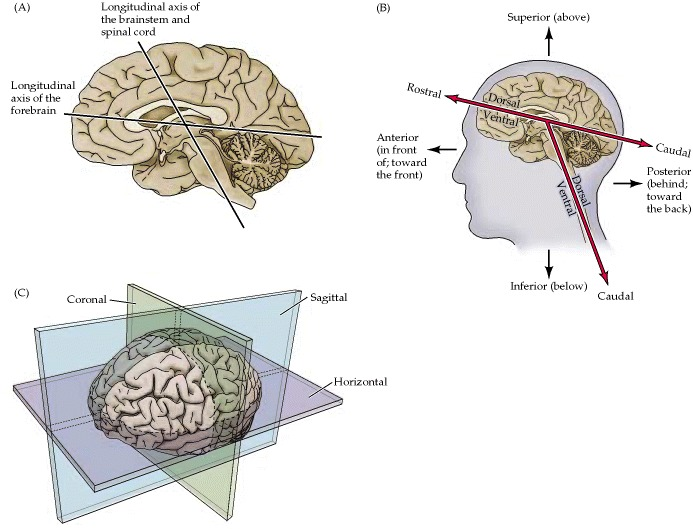
\includegraphics[scale=.6]{bilder/nervous_system.jpg}}%
           {Source: \url{https://www.ncbi.nlm.nih.gov/books/NBK10971/} , visited in September 2022.}
   
  \caption{Anatomical terminology. See (B). The terms anterior, posterior, superior, and inferior refer to the long axis of the body, while the terms dorsal, ventral, rostral, and caudal refer to the long axis of the central nervous system. Source: \url{https://www.ncbi.nlm.nih.gov/books/NBK10971/}, visited in September 2022.}
\end{figure}



%%% Local Variables:
%%% mode: latex
%%% TeX-master: "../thesis"
%%% End:
